% Presentazione Web Services ed ESB - Versione Discorsiva
% Autore: Prof. Fedeli Massimo
\documentclass{beamer}
\usetheme{Madrid}
\usecolortheme{default}
\usepackage[utf8]{inputenc}
\usepackage{graphicx}
\usepackage{tikz}
\usetikzlibrary{arrows.meta,shapes.geometric,positioning,shadows,calc,fit}
\usepackage{hyperref}
\usepackage{listings}
\usepackage{xcolor}

% Configurazione listing per XML
\lstdefinelanguage{XML}{
  basicstyle=\ttfamily\footnotesize,
  morestring=[b]",
  morestring=[s]{>}{<},
  morecomment=[s]{<?}{?>},
  stringstyle=\color{blue},
  identifierstyle=\color{red},
  keywordstyle=\color{orange},
  commentstyle=\color{green!50!black}
}

\title{Web Services e Enterprise Service Bus}
\subtitle{Architetture di Integrazione per Sistemi Distribuiti}
\author{Prof. Fedeli Massimo}
\institute{IIS Fermi Sacconi Ceci - Ascoli Piceno}
\date{}

\begin{document}

% Titolo
\begin{frame}
  \titlepage
\end{frame}

% Indice
\begin{frame}{Indice}
\tableofcontents
\end{frame}

\section{Introduzione}


\begin{frame}{L'evoluzione del Middleware}
Per comprendere appieno il valore dei Web Services, dobbiamo fare un passo indietro e osservare come sono evolute nel tempo le tecnologie di integrazione. Negli anni '80, il paradigma dominante era quello delle Remote Procedure Call (RPC), che permettevano di invocare funzioni su macchine remote come se fossero locali. Tuttavia, questo approccio presentava limiti significativi quando si trattava di integrare sistemi eterogenei.

\vspace{0.3cm}
Gli anni '90 hanno visto l'emergere di tecnologie più sofisticate come CORBA e DCOM, che promettevano interoperabilità multi-linguaggio e multi-piattaforma. Nonostante i progressi tecnologici, entrambe le soluzioni soffrivano di problemi con i firewall aziendali e di una complessità di configurazione che ne limitava l'adozione su larga scala.

\vspace{0.3cm}
L'avvento dei Web Services nei primi anni 2000 ha rappresentato una vera rivoluzione. Basandosi su standard aperti e sul protocollo HTTP, i Web Services hanno finalmente permesso un'integrazione efficace attraverso i confini organizzativi e tecnologici.
\end{frame}

\section{Middleware Tradizionali}

\begin{frame}{Il modello Client-Server e RPC}
Il \textbf{Remote Procedure Call} ha rappresentato uno dei primi tentativi di creare middleware per sistemi distribuiti. L'idea alla base era elegante nella sua semplicità: nascondere la complessità della rete al programmatore, permettendogli di chiamare una funzione remota esattamente come se fosse locale.

\vspace{0.3cm}
Questo approccio introduceva il concetto di \textit{\textbf{stub}} lato client e \textit{\textbf{skeleton}} lato server. Lo stub si occupava di serializzare i parametri della chiamata (marshalling) e inviarli attraverso la rete, mentre lo skeleton li deserializzava e invocava la funzione reale sul server. Il processo inverso gestiva il valore di ritorno.

\vspace{0.3cm}
Nonostante l'eleganza teorica, RPC presentava limiti pratici significativi. La \textbf{comunicazione sincrona bloccante} era problematica per sistemi ad alta latenza, mentre l'eterogeneità tecnologica e i firewall rappresentavano ostacoli quasi insormontabili nell'era di Internet.
\end{frame}

\begin{frame}{CORBA: l'ambizione dell'interoperabilità}
\textbf{CORBA} (Common Object Request Broker Architecture) rappresentò un tentativo ambizioso di creare un'infrastruttura universale per applicazioni distribuite orientate agli oggetti. Al centro dell'architettura stava l'Object Request Broker, un middleware intelligente capace di gestire la comunicazione tra oggetti distribuiti su reti eterogenee.

\vspace{0.3cm}
L'\textbf{IDL (Interface Definition Language) }permetteva di definire interfacce in modo neutrale rispetto al linguaggio di programmazione, generando automaticamente stub e skeleton per diversi linguaggi come C++, Java e Python. Il protocollo IIOP gestiva la comunicazione effettiva tra ORB diversi.

\vspace{0.3cm}
Nonostante le promesse iniziali, CORBA si è rivelato \textbf{complesso da configurare }e deployare. La necessità di porte dinamiche lo rendeva incompatibile con molte configurazioni firewall, limitandone l'uso principalmente a integrazioni intra-aziendali piuttosto che su Internet.
\end{frame}

\begin{frame}{COM e DCOM: l'ecosistema Microsoft}
In parallelo a CORBA, Microsoft sviluppava il proprio approccio ai componenti distribuiti con \textbf{COM (Component Object Model) }e la sua estensione distribuita DCOM. Profondamente integrato con Windows, COM offriva un modello elegante per la composizione di componenti software riutilizzabili.

\vspace{0.3cm}
\textbf{DCOM} estendeva questo modello attraverso la rete, permettendo a componenti su macchine diverse di collaborare come se fossero locali. Active Directory forniva meccanismi di discovery, mentre il Registry di Windows gestiva la registrazione dei componenti.

\vspace{0.3cm}
\end{frame}


\begin{frame}{NET Framework}
	\begin{itemize}
		\item Il limite principale di DCOM era la sua \textbf{natura proprietaria} e platform-dependent. 
		\item Funzionava eccellentemente all'interno di ecosistemi Windows omogenei, ma l'integrazione con altre piattaforme richiedeva soluzioni complesse e spesso inaffidabili.
		\item  \underline{Con l'avvento di .NET, Microsoft ha gradualmente} spostato l'attenzione verso architetture più aperte basate su Web Services.
	\end{itemize}

\end{frame}

\begin{frame}{Confronto tra i sistemi Middleware}
Osservando retrospettivamente queste tecnologie, emerge un quadro chiaro dei loro punti di forza e debolezza. 
\begin{itemize}
\item \textbf{CORBA} eccelleva nell'interoperabilità multi-linguaggio ma pagava un prezzo alto in termini di complessità. DCOM offriva prestazioni eccellenti e facilità d'uso nell'ecosistema Windows, ma era praticamente inutilizzabile al di fuori di esso.

\item 
Il problema comune a tutte queste soluzioni era il \textit{\textbf{tight coupling}}: le applicazioni dovevano conoscere dettagli implementativi l'una dell'altra e utilizzare protocolli specifici non standard. Inoltre, l'uso di formati binari proprietari e porte di rete dinamiche rendeva quasi impossibile l'attraversamento dei firewall.

\end{itemize}

\end{frame}


\begin{frame}{Confronto tra i sistemi Middleware}
	\vspace{0.3cm}
	I Web Services hanno risolto questi problemi adottando \textbf{XML} come formato di scambio universale, HTTP come protocollo di trasporto firewall-friendly, e standard aperti definiti da W3C e OASIS. 
	
	Questo ha permesso finalmente di realizzare l'integrazione veramente universale che le tecnologie precedenti avevano solo promesso.
\end{frame}

\section{XML e Standard Web Services}

\begin{frame}{XML: il fondamento dei Web Services}
\textbf{XML (eXtensible Markup Language) }ha giocato un ruolo centrale nel successo dei Web Services. A differenza dei formati binari proprietari usati da CORBA e DCOM, XML è \underline{testuale, human-readable e completamente estensibile}. Questo lo rende ideale per la comunicazione tra sistemi eterogenei.

\vspace{0.3cm}
La forza di XML sta nella sua capacità di essere contemporaneamente semplice e potente. Attraverso i namespaces, permette di combinare vocabolari diversi senza conflitti. Con gli schemi XSD, offre validazione formale della struttura dei documenti, garantendo che mittente e destinatario condividano la stessa comprensione dei dati scambiati.
\end{frame}


\begin{frame}{XML: il fondamento dei Web Services}
	
	\vspace{0.3cm}
	Nei Web Services, XML viene utilizzato a più livelli: per i messaggi \textbf{SOAP} che trasportano i dati, per i documenti \textbf{WSDL} che descrivono le interfacce, per i registry \textbf{UDDI} che catalogano i servizi disponibili. Questa uniformità semplifica notevolmente l'implementazione e il debugging dei sistemi integrati.
\end{frame}



\begin{frame}{SOAP: il protocollo universale}
\textbf{SOAP} (Simple Object Access Protocol) rappresenta il protocollo standard per lo scambio di messaggi tra Web Services. Nonostante il nome, SOAP non è particolarmente semplice, ma offre una struttura robusta e estensibile per la comunicazione distribuita.

\vspace{0.3cm}
Un messaggio SOAP è fondamentalmente un documento XML strutturato in tre parti principali. L'\textit{Envelope} funge da contenitore root, dichiarando che il documento è un messaggio SOAP. L'\textit{Header} opzionale trasporta metadati come informazioni di autenticazione, routing o gestione delle transazioni. Il \textit{Body} contiene il payload effettivo, che può essere una chiamata RPC o un documento strutturato.

\vspace{0.3cm}
Una caratteristica fondamentale di SOAP è il suo essere stateless: ogni richiesta è autocontenuta e non dipende da richieste precedenti. Questo semplifica notevolmente la scalabilità e l'affidabilità dei sistemi, permettendo tecniche come il load balancing senza necessità di session affinity.
\end{frame}

\begin{frame}{Anatomia di un messaggio SOAP}
\begin{center}
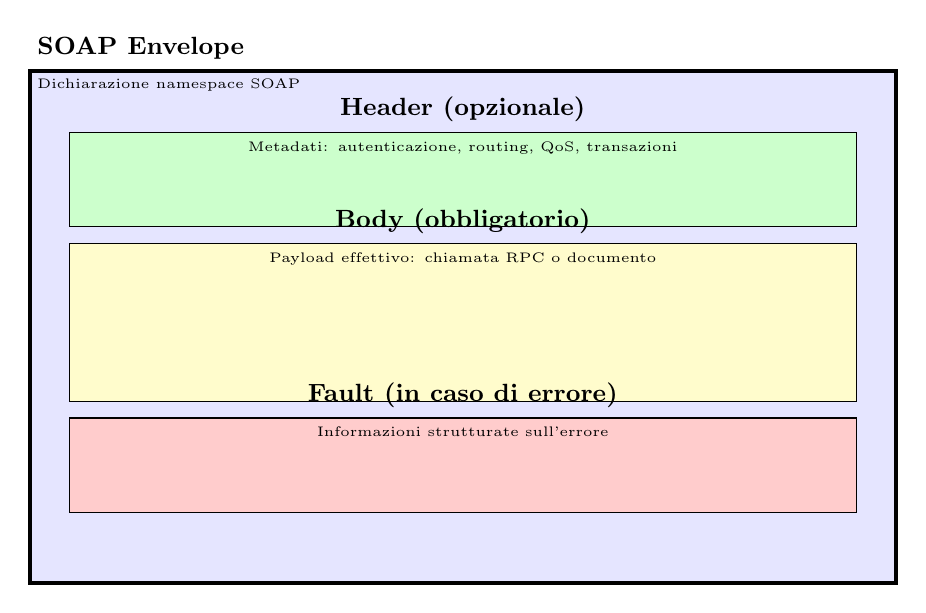
\begin{tikzpicture}[node distance=0mm, every node/.style={font=\small}]
\node[draw,rectangle,minimum width=11cm,minimum height=6.5cm,fill=blue!10,line width=1.5pt] (env) {};
\node[above right] at (env.north west) {\textbf{SOAP Envelope}};
\node[below right,font=\tiny] at (env.north west) {Dichiarazione namespace SOAP};

\node[draw,rectangle,below=8mm of env.north,minimum width=10cm,minimum height=1.2cm,fill=green!20] (hdr) {};
\node[above] at (hdr.north) {\textbf{Header (opzionale)}};
\node[below,font=\tiny,text width=9cm,align=center] at (hdr.north) {
Metadati: autenticazione, routing, QoS, transazioni
};

\node[draw,rectangle,below=2mm of hdr,minimum width=10cm,minimum height=2cm,fill=yellow!20] (body) {};
\node[above] at (body.north) {\textbf{Body (obbligatorio)}};
\node[below,font=\tiny,text width=9cm,align=center] at (body.north) {
Payload effettivo: chiamata RPC o documento
};

\node[draw,rectangle,below=2mm of body,minimum width=10cm,minimum height=1.2cm,fill=red!20] (fault) {};
\node[above] at (fault.north) {\textbf{Fault (in caso di errore)}};
\node[below,font=\tiny,text width=9cm,align=center] at (fault.north) {
Informazioni strutturate sull'errore
};
\end{tikzpicture}
\end{center}
\end{frame}

\begin{frame}[fragile]{Un esempio concreto di messaggio SOAP}
Vediamo ora un esempio pratico di come appare un messaggio SOAP nel mondo reale. Immaginiamo di voler interrogare un servizio finanziario per ottenere l'ultimo prezzo di un'azione.

\begin{lstlisting}[language=XML,basicstyle=\ttfamily\tiny]
<?xml version="1.0"?>
<soap:Envelope 
  xmlns:soap="http://schemas.xmlsoap.org/soap/envelope/">
  
  <soap:Header>
    <m:Authentication xmlns:m="http://www.stock.org/stock">
      <m:Token>Bearer abc123xyz</m:Token>
    </m:Authentication>
  </soap:Header>
  
  <soap:Body>
    <m:GetLastTradePrice xmlns:m="http://www.stock.org/stock">
      <m:Symbol>AAPL</m:Symbol>
    </m:GetLastTradePrice>
  </soap:Body>
</soap:Envelope>
\end{lstlisting}

\vspace{0.2cm}
Questo messaggio verrebbe inviato via HTTP POST all'endpoint del servizio, che risponderebbe con un altro messaggio SOAP contenente il prezzo richiesto.
\end{frame}

\begin{frame}{Document-style vs RPC-style}
\textbf{SOAP} supporta due stili fondamentali di interazione che riflettono filosofie diverse di comunicazione distribuita. Lo stile\textbf{ RPC (Remote Procedure Call)} modella la comunicazione come una chiamata di funzione: invio parametri e ricevo un valore di ritorno. È \textbf{sincrono} per natura e crea un accoppiamento più stretto tra client e server.

\vspace{0.3cm}
Lo stile \textbf{Document}, invece, concepisce la comunicazione come uno scambio di documenti XML. Il client invia un documento che descrive un'azione da compiere, e il server può rispondere o meno. Questo approccio è naturalmente più adatto alla comunicazione asincrona e al \textbf{loose coupling}.

\end{frame}


\begin{frame}{Document-style vs RPC-style}
	
	\vspace{0.3cm}
	Nella pratica, lo stile \textbf{Document/Literal Wrapped} è diventato lo standard de facto. Combina la semplicità concettuale dell'RPC con i vantaggi della validazione XSD del document-style. È questo lo stile che si trova implementato nella maggior parte dei framework moderni come Apache CXF o Spring WS.
\end{frame}

\begin{frame}{Gestione degli errori con SOAP Fault}
Anche i sistemi meglio progettati incontrano errori, e SOAP fornisce un meccanismo strutturato per comunicarli attraverso l'elemento Fault. Quando un servizio non può completare una richiesta, invece di restituire un normale messaggio di risposta, restituisce un \textbf{Fault} nel body del messaggio SOAP.

\vspace{0.3cm}
La struttura del Fault è standardizzata e include diversi elementi informativi. Il \textit{faultcode} categorizza l'errore in classi standard come VersionMismatch, MustUnderstand, Client o Server. Il \textit{faultstring} fornisce una descrizione human-readable dell'errore. L'elemento \textit{detail} può contenere informazioni specifiche dell'applicazione sull'errore verificatosi.

\end{frame}


\begin{frame}{Gestione degli errori con SOAP Fault}
	
	\vspace{0.3cm}
	Questa standardizzazione permette ai client di implementare logiche di \textbf{retry, fallback} o compensazione in modo consistente, indipendentemente dal servizio specifico che stanno invocando. È un esempio di come gli standard ben progettati facilitino l'interoperabilità.
\end{frame}


\section{WSDL e Discovery}

\begin{frame}{WSDL: il contratto tra servizi}
Se SOAP definisce come i messaggi vengono strutturati, \textbf{WSDL} (Web Services Description Language) definisce quali messaggi un servizio può accettare e produrre. È essenzialmente un contratto machine-readable che descrive completamente l'interfaccia di un Web Service.

\vspace{0.3cm}
La bellezza di WSDL sta nella sua struttura a due livelli. La parte astratta descrive cosa il servizio fa: quali operazioni offre, quali messaggi accetta e restituisce, quali tipi di dati utilizza. Questa parte è indipendente da come il servizio è effettivamente implementato o esposto.

\vspace{0.3cm}
La parte concreta, invece, specifica i dettagli implementativi: quale protocollo viene usato (tipicamente SOAP su HTTP), quale formato di encoding, e soprattutto dove il servizio è fisicamente disponibile (l'URL dell'endpoint). Questa separazione permette di cambiare l'implementazione senza modificare l'interfaccia logica.
\end{frame}

%\begin{frame}{La struttura di un documento WSDL}
%	\begin{center}
%		\begin{tikzpicture}[
%			node distance=1.5cm,
%			box/.style={draw,rectangle,minimum width=2.5cm,minimum height=0.8cm,rounded corners,font=\small},
%			abstract/.style={fill=blue!20},
%			concrete/.style={fill=orange!20}
%			]
%			\node[box,abstract] (types) {Types\\(XSD)};
%			\node[box,abstract,right=of types] (message) {Message\\(parts)};
%			\node[box,abstract,right=of message] (operation) {Operation\\(I/O)};
%			\node[box,abstract,right=of operation] (porttype) {PortType\\(Interface)};
%			\node[box,concrete,below=2cm of porttype] (binding) {Binding\\(Protocol)};
%			\node[box,concrete,below=of binding] (port) {Port\\(Endpoint)};
%			\node[box,concrete,below=of port] (service) {Service\\(Collection)};
%			
%			\draw[-{Stealth},thick] (types) -- (message) node[midway,above,font=\tiny] {usa};
%			\draw[-{Stealth},thick] (message) -- (operation) node[midway,above,font=\tiny] {compone};
%			\draw[-{Stealth},thick] (operation) -- (porttype) node[midway,above,font=\tiny] {raggruppa};
%			\draw[-{Stealth},thick] (porttype) -- (binding) node[midway,right,font=\tiny] {implementa};
%			\draw[-{Stealth},thick] (binding) -- (port) node[midway,right,font=\tiny] {specifica};
%			\draw[-{Stealth},thick] (port) -- (service) node[midway,right,font=\tiny] {espone};
%			
%			\node[left=0.3cm of types,rotate=90,font=\small,blue] {ASTRATTO};
%			\node[left=0.3cm of binding,rotate=90,font=\small,orange] {CONCRETO};
%			
%			\draw[dashed,thick,gray] ($(types.south west)+(-0.5,-0.8)$) -- ($(porttype.south east)+(0.5,-0.8)$);
%		\end{tikzpicture}
%	\end{center}
%\end{frame}

\begin{frame}{L'utilizzo pratico del WSDL}
Il vero potere del WSDL emerge quando lo si usa per generare automaticamente il codice client. I moderni framework di Web Services possono leggere un documento WSDL e generare proxy client completamente tipizzati nel linguaggio di programmazione scelto.

\vspace{0.3cm}
In Java, strumenti come wsimport o Apache CXF possono trasformare un WSDL in classi Java che rappresentano le operazioni del servizio come metodi. In .NET, Visual Studio offre la funzionalità ``Add Service Reference'' che genera automaticamente il codice necessario. Anche linguaggi dinamici come Python hanno librerie come zeep che semplificano enormemente l'interazione con Web Services.

\vspace{0.3cm}
Questo approccio ``contract-first'' porta numerosi vantaggi. Gli errori vengono catturati a compile-time piuttosto che a runtime. La documentazione è sempre allineata con l'implementazione. E soprattutto, client e server possono essere sviluppati in parallelo una volta che il contratto WSDL è stato definito.
\end{frame}

\begin{frame}{UDDI: le Pagine Gialle dei servizi}
Con SOAP che definisce come comunicare e WSDL che descrive cosa comunicare, mancava ancora un pezzo: come scoprire quali servizi esistono. \textbf{UDDI} (Universal Description, Discovery and Integration) fu concepito come un registry distribuito, una sorta di ``Pagine Gialle'' per Web Services.

\vspace{0.3cm}
L'idea era elegante: le aziende avrebbero pubblicato i loro servizi in registry \textbf{UDDI pubblici o privati}, completi di informazioni di business (White Pages), categorizzazione per industria e geografia (Yellow Pages), e dettagli tecnici come i link ai WSDL (Green Pages). I potenziali consumatori avrebbero potuto cercare servizi per categoria o caratteristica e scoprire dinamicamente i provider.

\end{frame}


\begin{frame}{UDDI: le Pagine Gialle dei servizi}

	\vspace{0.3cm}
	Nella pratica, i registry UDDI pubblici hanno avuto vita breve. La complessità del protocollo, i problemi di spam e la mancanza di un modello di business sostenibile hanno portato alla chiusura dei principali registry pubblici entro il 2006. Tuttavia, il concetto vive ancora nei registry privati enterprise e nelle moderne API management platform.
\end{frame}



\begin{frame}{WSIL: un'alternativa pragmatica}
Di fronte alla complessità e all'insuccesso di UDDI, emerse un'alternativa più semplice chiamata \textbf{WSIL} (Web Services Inspection Language). Invece di un registry centralizzato complesso, WSIL propone un approccio decentralizzato e minimale.

\vspace{0.3cm}
L'idea è semplicemente quella di avere un file XML standard (tipicamente chiamato \texttt{inspection.wsil}) nella root di un web server. Questo file contiene link ai WSDL dei servizi disponibili su quel server, insieme a metadati basilari. I file WSIL possono anche contenere link ad altri file WSIL, creando una rete di discovery distribuita.

\vspace{0.3cm}
WSIL non ha mai raggiunto l'adozione di massa, ma ha influenzato approcci successivi come le API directories e i service catalogs delle piattaforme cloud moderne. La lezione appresa è che spesso le soluzioni semplici e decentralizzate funzionano meglio delle architetture complesse centralizzate.
\end{frame}

\section{Performance e Tecnologie Avanzate}

\begin{frame}{Le prestazioni dei Web Services}
Una critica frequente ai Web Services SOAP riguarda le prestazioni. E in effetti, confrontati con protocolli binari come CORBA o con REST/JSON moderni, SOAP presenta overhead significativi. L'XML è verboso, il parsing richiede risorse, e l'incapsulamento in SOAP aggiunge ulteriori byte ad ogni messaggio.

\vspace{0.3cm}
Tuttavia, questa analisi va contestualizzata. Per messaggi piccoli e frequenti, l'overhead può essere problematico. Ma per transazioni enterprise complesse, dove il processing logico domina sul tempo di rete, la differenza diventa marginale. Inoltre, molte delle funzionalità enterprise che SOAP fornisce nativamente (sicurezza, transazioni, reliable messaging) devono essere implementate manualmente in soluzioni più leggere.

\vspace{0.3cm}
Esistono comunque diverse strategie di ottimizzazione. La compressione HTTP può ridurre drasticamente la dimensione dei messaggi. MTOM (Message Transmission Optimization Mechanism) permette di trasmettere dati binari efficientemente. Il caching intelligente delle risposte e l'uso di connessioni persistenti HTTP/1.1 possono migliorare significativamente il throughput.
\end{frame}

\begin{frame}{Il ciclo di hype e maturazione}
È interessante osservare la traiettoria dei Web Services attraverso la lente del Gartner Hype Cycle. Nei primi anni 2000, l'entusiasmo era alle stelle: Web Services erano visti come la soluzione definitiva a tutti i problemi di integrazione. Ogni vendor tecnologico promuoveva la propria implementazione SOAP.

\vspace{0.3cm}
Poi arrivò la disillusione. La complessità dello stack WS-*, le questioni di performance, e l'emergere di REST come alternativa più semplice portarono molti a dichiarare i Web Services morti. Era il classico ``trough of disillusionment'' del ciclo di hype.

\vspace{0.3cm}
Oggi ci troviamo nel ``plateau of productivity''. Web Services SOAP non sono morti, ma hanno trovato la loro nicchia: sistemi enterprise mission-critical dove affidabilità, sicurezza e standard rigorosi sono più importanti della semplicità o delle prestazioni pure. Convivono pacificamente con REST per scenari più semplici e con tecnologie più moderne come gRPC per casi ad alte prestazioni.
\end{frame}

\begin{frame}{BPEL: orchestrare i servizi}
I singoli Web Services sono utili, ma il vero potere emerge quando li si orchestra in processi di business complessi. BPEL (Business Process Execution Language) fu creato proprio per questo scopo: permettere di definire workflow che coordinano l'invocazione di multipli Web Services.

\vspace{0.3cm}
BPEL è essenzialmente un linguaggio di programmazione XML-based specializzato per l'orchestrazione. Offre costrutti per sequenze, decisioni condizionali, cicli, esecuzione parallela, gestione delle eccezioni e compensazioni. Ogni servizio coinvolto nel processo è descritto tramite il suo WSDL, garantendo type-safety e verificabilità.

\vspace{0.3cm}
Un motore BPEL esegue questi processi, gestendo lo stato, le transazioni e la comunicazione con i servizi. Questo approccio è particolarmente potente per processi long-running che possono durare giorni o settimane, dove la persistenza dello stato e la capacità di recupero da errori sono cruciali.
\end{frame}

\begin{frame}{Orchestrazione vs Coreografia}
Quando si coordinano multipli servizi, emergono due paradigmi architetturali fondamentalmente diversi. Nell'orchestrazione, un componente centrale (l'orchestratore) ha la visione globale del processo e coordina tutti i servizi partecipanti. È come un direttore d'orchestra che coordina i musicisti.

\vspace{0.3cm}
La coreografia, invece, è un approccio peer-to-peer dove non c'è un coordinatore centrale. Ogni servizio conosce le proprie responsabilità e risponde agli eventi appropriati. È più simile a una danza dove ogni ballerino conosce i propri passi e si coordina osservando gli altri.

\vspace{0.3cm}
L'orchestrazione è più semplice da implementare e monitorare, ma crea un single point of failure. La coreografia è più resiliente e scalabile, ma più complessa da debuggare e comprendere. Nella pratica, molti sistemi usano un approccio ibrido, con orchestrazione locale all'interno di confini organizzativi e coreografia tra organizzazioni diverse.
\end{frame}

\begin{frame}{Il pattern Find-Bind-Invoke}
Uno dei concetti fondamentali dell'architettura SOA è il pattern Find-Bind-Invoke, che descrive il ciclo di vita completo dell'interazione con un servizio. Inizia con la fase di discovery (Find), dove un potenziale consumer cerca servizi che soddisfano le sue esigenze, tipicamente usando un registry come UDDI.

\vspace{0.3cm}
Una volta trovato un servizio appropriato, il consumer ottiene il suo WSDL e genera il codice client necessario (Bind). Questo può avvenire a compile-time (binding statico) o a runtime (binding dinamico), a seconda delle esigenze dell'applicazione.

\vspace{0.3cm}
Infine, il consumer invoca effettivamente il servizio (Invoke), inviando messaggi SOAP all'endpoint specificato nel WSDL. Questo pattern, sebbene concepito originariamente per Web Services, rimane rilevante anche in architetture più moderne basate su microservizi e service mesh.
\end{frame}

\begin{frame}{Sicurezza nei Web Services}
La sicurezza nei Web Services opera a due livelli complementari. La sicurezza a livello di trasporto, tipicamente HTTPS/TLS, protegge i messaggi mentre viaggiano sulla rete, ma solo punto-a-punto. Se un messaggio attraversa intermediari, ogni hop deve essere protetto separatamente.

\vspace{0.3cm}
La sicurezza a livello di messaggio, implementata attraverso WS-Security, offre protezione end-to-end. Il messaggio può essere firmato digitalmente per garantire integrità e non-ripudio, e cifrato per confidenzialità. Parti diverse del messaggio possono avere livelli di sicurezza diversi, e la sicurezza persiste attraverso intermediari.

\vspace{0.3cm}
WS-Security supporta vari tipi di token di sicurezza: username/password, certificati X.509, token SAML per single sign-on, e ticket Kerberos. Questa flessibilità permette di integrare Web Services in complesse infrastrutture di sicurezza enterprise già esistenti.
\end{frame}

\begin{frame}{Lo stack WS-*: potenza e complessità}
Oltre a SOAP, WSDL e WS-Security, esiste un'intera famiglia di specifiche note collettivamente come WS-* (``WS-star''). Ciascuna affronta un aspetto specifico delle applicazioni enterprise distribuite.

\vspace{0.3cm}
WS-ReliableMessaging garantisce la consegna dei messaggi anche in presenza di fallimenti di rete. WS-AtomicTransaction estende il modello transazionale ACID a Web Services distribuiti. WS-Policy permette di dichiarare requisiti e capacità in modo machine-readable. WS-Addressing fornisce meccanismi di indirizzamento endpoint-neutral.

\vspace{0.3cm}
La critica principale allo stack WS-* è la sua complessità. Implementare correttamente tutte queste specifiche richiede framework sofisticati e competenze specializzate. Tuttavia, per sistemi enterprise mission-critical in settori regolamentati come finanza o sanità, questa complessità è spesso giustificata dai requisiti di affidabilità, sicurezza e compliance.
\end{frame}

\section{Enterprise Application Integration}

\begin{frame}{Il problema dell'integrazione enterprise}
Le grandi organizzazioni accumulano nel tempo un ecosistema eterogeneo di applicazioni: sistemi ERP, CRM, SCM, legacy mainframe, warehouse, e molto altro. Ciascuna di queste applicazioni ha il proprio database, il proprio formato dati, e la propria logica di business. Il problema è farle collaborare efficacemente.

\vspace{0.3cm}
L'approccio più naive è l'integrazione point-to-point: creare connessioni dirette tra ogni coppia di sistemi che devono comunicare. Questo scala malissimo: con N sistemi, potresti aver bisogno di N*(N-1)/2 connessioni. Ogni nuova applicazione o modifica richiede cambiamenti a molteplici integrazioni.

\vspace{0.3cm}
Da questo problema nasce l'Enterprise Application Integration (EAI), un insieme di approcci e tecnologie per gestire sistematicamente l'integrazione. L'obiettivo è ridurre il coupling, centralizzare la logica di integrazione, e rendere l'aggiunta di nuove applicazioni il più indolore possibile.
\end{frame}

\begin{frame}{Hub-and-Spoke: centralizzazione}
Il primo approccio EAI maturo fu l'architettura Hub-and-Spoke. Invece di connessioni point-to-point, tutte le applicazioni si connettono a un hub centrale che gestisce routing, trasformazione e orchestrazione dei messaggi.

\vspace{0.3cm}
Questo riduce drasticamente il numero di connessioni: da O(N²) a O(N). Ogni applicazione deve solo sapere come comunicare con l'hub, non con tutte le altre applicazioni. Le logiche di trasformazione dati e routing sono centralizzate, facilitando manutenzione e governance.

\vspace{0.3cm}
Tuttavia, l'hub-and-spoke ha un tallone d'Achille: l'hub stesso diventa un single point of failure e un potenziale collo di bottiglia. Con volumi di traffico elevati, l'hub può saturarsi. La ridondanza richiede complessi meccanismi di sincronizzazione dello stato. Questi limiti hanno portato all'evoluzione verso architetture bus.
\end{frame}

\begin{frame}{Verso il Bus di integrazione}
L'architettura a bus risolve i problemi dell'hub-and-spoke distribuendo il carico su multipli nodi. Invece di un hub monolitico centrale, si ha un'infrastruttura logicamente unificata ma fisicamente distribuita. Le applicazioni si connettono a nodi del bus che possono essere replicati e distribuiti geograficamente.

\vspace{0.3cm}
Questa distribuzione porta resilienza: il fallimento di un nodo non paralizza l'intero sistema. Porta anche scalabilità: si possono aggiungere nodi per gestire carichi crescenti. E porta flessibilità: nodi diversi possono specializzarsi in task diversi (trasformazioni, routing, protocolli specifici).

\vspace{0.3cm}
Il prezzo da pagare è una maggiore complessità operativa. La configurazione deve essere sincronizzata tra nodi. Il monitoring diventa più complesso. Il debugging di problemi può richiedere la tracciatura di messaggi attraverso multipli nodi. Ma per organizzazioni enterprise con requisiti di alta disponibilità, questi trade-off sono generalmente accettabili.
\end{frame}

\section{Enterprise Service Bus}

\begin{frame}{ESB: l'evoluzione dell'integrazione}
L'Enterprise Service Bus rappresenta l'apice dell'evoluzione delle tecnologie EAI, combinando le migliori idee dell'architettura a bus con gli standard dei Web Services e i principi SOA. Un ESB non è solo un prodotto ma un pattern architetturale per costruire infrastrutture di integrazione moderne.

\vspace{0.3cm}
Al cuore dell'ESB c'è il concetto di mediation: l'ESB si interpone tra servizi, fornendo servizi di valore aggiunto come routing intelligente, trasformazione dati, protocol bridging, sicurezza, transazioni, e molto altro. I servizi connessi all'ESB non devono conoscere i dettagli implementativi degli altri servizi: l'ESB gestisce tutte le complessità di integrazione.

\vspace{0.3cm}
Questa mediazione permette di sostituire facilmente implementazioni di servizi, aggiungere nuovi consumer o provider, cambiare protocolli di comunicazione, tutto senza impattare i servizi esistenti. L'ESB diventa la spina dorsale dell'infrastruttura IT enterprise, permettendo agilità in un contesto altrimenti rigido di sistemi legacy.
\end{frame}

\begin{frame}{Le funzionalità core dell'ESB}
Un ESB moderno offre un ricco set di funzionalità che vanno ben oltre il semplice routing di messaggi. Il routing stesso può essere content-based: l'ESB esamina il contenuto del messaggio e decide dinamicamente quale servizio deve gestirlo, permettendo implementazioni sofisticate di business rules.

\vspace{0.3cm}
La trasformazione dati è centrale: sistemi diversi parlano linguaggi diversi, e l'ESB traduce tra formati. XSLT per trasformazioni XML, mapper visulai per logiche complesse, enrichment per arricchire messaggi con dati da database o altri servizi, aggregation per combinare risposte da multipli servizi.

\vspace{0.3cm}
Protocol mediation permette a sistemi che parlano protocolli diversi di comunicare attraverso l'ESB. Un sistema legacy che usa FTP può comunicare con un moderno REST API senza che nessuno dei due debba cambiare. L'ESB gestisce la conversione del protocollo in modo trasparente.
\end{frame}

\begin{frame}{Message-Oriented Middleware}
La maggior parte degli ESB moderni si basa su Message-Oriented Middleware (MOM) per la comunicazione asincrona. Il MOM fornisce due modelli fondamentali: le code (queue) per comunicazione point-to-point e i topic per publish-subscribe.

\vspace{0.3cm}
Con le queue, un producer invia messaggi a una coda e uno o più consumer li prelevano per processarli. Se ci sono multipli consumer, ciascun messaggio va a uno solo di essi, permettendo load balancing automatico. I messaggi persistono nella coda finché non vengono consumati, garantendo che non si perdano anche se i consumer sono temporaneamente indisponibili.

\vspace{0.3cm}
I topic implementano il pattern publish-subscribe: un publisher invia messaggi a un topic, e tutti i subscriber interessati ricevono una copia. Questo è ideale per event notification e broadcasting. La separazione tra publisher e subscriber permette di aggiungere nuovi subscriber senza modificare il publisher.
\end{frame}

\begin{frame}{JBI: uno standard per ESB}
Java Business Integration (JSR 208) fu un tentativo di standardizzare l'architettura degli ESB nel mondo Java. L'idea era permettere di creare ESB componendo componenti da vendor diversi, garantendo interoperabilità attraverso un'architettura plugin standard.

\vspace{0.3cm}
Al centro di JBI sta il Normalized Message Router (NMR), un bus interno che gestisce lo scambio di messaggi in formato canonico. I componenti si dividono in Service Engine (che implementano logica di business come BPEL o trasformazioni XSLT) e Binding Components (che gestiscono protocolli esterni come SOAP, JMS, FTP).

\vspace{0.3cm}
Sebbene JBI abbia avuto adozione limitata e sia stato superato da approcci più moderni, i suoi concetti rimangono influenti. L'idea di normalizzare i messaggi all'ingresso del bus e di separare logica di business da protocol handling sono best practices ancora rilevanti negli ESB contemporanei.
\end{frame}

\begin{frame}{Pattern di scambio messaggi}
Gli ESB supportano diversi pattern di scambio messaggi (Message Exchange Patterns) che codificano le aspettative di comunicazione. Il pattern più semplice è In-Only: il consumer invia un messaggio e non attende risposta. È fire-and-forget, utile per notifiche e logging.

\vspace{0.3cm}
Robust In-Only aggiunge acknowledgment: il provider conferma la ricezione o segnala un errore, ma non restituisce dati di business. In-Out è il classico request-response: il consumer invia una richiesta e attende una risposta. Può essere implementato sincronamente o asincronamente tramite code.

\vspace{0.3cm}
In Optional-Out è un pattern più flessibile dove il provider può decidere se rispondere o meno basandosi sulla logica di business. Questi pattern formalizzano aspettative e obblighi, permettendo agli ESB di gestire correttamente timeout, retry, e error handling in modo appropriato per ciascun pattern.
\end{frame}

\begin{frame}{Routing e trasformazione: il cuore dell'ESB}
Il routing intelligente è ciò che rende un ESB più di un semplice message broker. Content-based routing esamina il payload del messaggio per decidere la destinazione: ordini sotto mille euro vanno al sistema automatico, sopra richiedono approvazione manuale. Header-based routing usa metadati per routing più efficiente senza parsare il payload.

\vspace{0.3cm}
La trasformazione è ugualmente cruciale. Due sistemi raramente parlano esattamente lo stesso linguaggio. L'ESB trasforma messaggi in transito: formato XML del sistema A diventa JSON per sistema B. Campo ``customer\_id'' diventa ``clientCode''. Date da formato europeo a ISO. Valute convertite.

\vspace{0.3cm}
Enrichment arricchisce messaggi con dati addizionali: un ordine contiene solo l'ID cliente, l'ESB fa lookup nel database clienti e aggiunge nome, indirizzo, credito disponibile prima di inoltrarlo al sistema di fulfillment. Splitting divide messaggi complessi in multipli messaggi semplici. Aggregation fa l'opposto.
\end{frame}

\begin{frame}{Monitoraggio e osservabilità}
Un ESB in produzione gestisce potenzialmente migliaia di messaggi al secondo attraverso decine di servizi. Senza monitoraggio adeguato, diagnosticare problemi diventa impossibile. I moderni ESB implementano comprehensive logging: ogni messaggio può essere loggato con correlation ID che permette di tracciarlo attraverso l'intero flusso.

\vspace{0.3cm}
Le metriche real-time sono essenziali: throughput per servizio, latenze percentili (p50, p95, p99), error rates, queue depths. Dashboard visualizzano lo stato del sistema a colpo d'occhio. Alert automatici notificano quando metriche violano soglie: latenza troppo alta, error rate in crescita, code che si riempiono.

\vspace{0.3cm}
Il tracing distribuito permette di seguire un singolo messaggio attraverso multipli servizi e trasformazioni. Quando un utente lamenta un ordine perso, si può cercare per transaction ID e vedere esattamente dove il messaggio si è fermato, quale trasformazione è fallita, quale servizio ha restituito errore.
\end{frame}

\begin{frame}{Scalabilità e resilienza}
Gli ESB production-grade devono gestire volumi enormi mantenendo alta disponibilità. La scalabilità orizzontale è fondamentale: quando il carico cresce, si aggiungono nodi ESB al cluster. Load balancer distribuiscono il traffico. Code distribuite permettono a qualsiasi nodo di processare qualsiasi messaggio.

\vspace{0.3cm}
La resilienza richiede strategie multiple. Circuit breaker previene cascading failures: se un servizio inizia a fallire, il circuit breaker lo ``apre'', fermando tentativi che fallirebbero comunque e dando al servizio tempo di recuperare. Retry logic con exponential backoff gestisce fallimenti transienti. Timeout prevengono che richieste lente blocchino risorse.

\vspace{0.3cm}
Bulkhead isolation isola fallimenti: problemi in un'area non propagano ad altre. Se il servizio di fatturazione è sovraccarico, l'isolamento garantisce che ordini e spedizioni continuino a funzionare. Geographic redundancy permette failover automatico se un datacenter diventa indisponibile.
\end{frame}

\section{Casi d'Uso e Best Practices}

\begin{frame}{Integrazione CRM-ERP}
Consideriamo un caso d'uso pratico che illustra il valore dell'ESB. Un'azienda ha un sistema CRM dove il team vendite crea ordini, e un sistema ERP che gestisce inventario, produzione e fatturazione. Questi sistemi devono rimanere sincronizzati, ma sono stati acquistati da vendor diversi e non parlano lo stesso linguaggio.

\vspace{0.3cm}
Quando un ordine viene creato nel CRM, scatena un evento che l'ESB intercetta. L'ESB valida l'ordine contro regole di business, arricchisce i dati consultando il database clienti per informazioni fiscali, trasforma il formato CRM nel formato che l'ERP comprende, e invoca il servizio ERP per creare l'ordine.

\vspace{0.3cm}
Se l'ERP conferma successo, l'ESB aggiorna lo stato nel CRM e invia email di conferma al cliente. Se fallisce, l'ESB può ritentare automaticamente, loggare l'errore per investigazione, e notificare il team ops. Tutto questo senza che CRM ed ERP debbano conoscersi direttamente.
\end{frame}

\begin{frame}{Compensating transactions}
In sistemi distribuiti, non possiamo avere transazioni ACID tradizionali che coinvolgono multipli servizi esterni. Se prenotiamo un volo, poi un hotel, poi un'auto, e la prenotazione auto fallisce, dobbiamo ``disfare'' le prenotazioni precedenti.

\vspace{0.3cm}
Il pattern Saga risolve questo problema: ogni operazione ha una compensazione che la annulla. Se la sequenza completa ha successo, tutto bene. Se un passo fallisce, eseguiamo le compensazioni in ordine inverso. Prenotato volo, prenotato hotel, fallita auto: compensiamo cancellando hotel, poi cancellando volo.

\vspace{0.3cm}
Le compensazioni non sono sempre perfette. Cancellare una prenotazione potrebbe avere penali. Alcuni cambiamenti non sono reversibili. Ma in assenza di transazioni distribuite, i Saga rappresentano un compromesso pratico che permette di mantenere consistenza eventuale in sistemi distribuiti complessi.
\end{frame}

\begin{frame}{Testing e CI/CD}
I Web Services e gli ESB pongono sfide uniche per testing e deployment. Unit testing è relativamente semplice: si mockano le dipendenze e si testano componenti isolati. Contract testing verifica che client e server concordino sull'interfaccia: il WSDL è il contratto.

\vspace{0.3cm}
Integration testing diventa complesso: servizi reali potrebbero non essere disponibili in ambiente di test, o potrebbero avere rate limits, o costare denaro per chiamata. Service virtualization risolve questo creando mock services che simulano comportamento reale includendo latenze, errori occasionali, e variazioni di risposta.

\vspace{0.3cm}
La pipeline CI/CD per servizi include validazione WSDL, generazione e test di stub, deployment a staging con smoke tests, monitoraggio post-deployment. Blue-green deployment o canary releases permettono rollback veloce se problemi emergono in produzione. L'automazione è cruciale per mantenere qualità con deployment frequenti.
\end{frame}

\begin{frame}{Strategia di migrazione}
Sostituire integrazioni point-to-point legacy con un ESB non può essere big-bang: troppo rischioso e disruptive. L'approccio pragmatico è incrementale, spesso chiamato Strangler Fig Pattern dal modo in cui alcune piante crescono attorno ad alberi esistenti.

\vspace{0.3cm}
Si inizia con assessment: catalogare integrazioni esistenti, identificare pain points, prioritizzare per valore e rischio. Si seleziona un pilot: un'integrazione importante ma non critica, con stakeholder supportivi. Si implementa nel nuovo ESB, si testa exhaustivamente, si monitora in parallelo al vecchio sistema.

\vspace{0.3cm}
Con successo validato, si espande progressivamente. Nuove integrazioni vanno direttamente su ESB. Integrazioni esistenti migrano quando opportuno: quando richiedono modifiche, o quando obsolescenza tecnologica lo rende necessario. Nel tempo, il vecchio si riduce e il nuovo domina, senza mai un cutover rischioso.
\end{frame}

\begin{frame}{Best practices architetturali}
L'esperienza collettiva dell'industria ha cristallizzato alcune best practices fondamentali. Design for failure: assumete che ogni componente fallirà, e progettate per resilienza. Circuit breakers, timeout, retry, fallback: non opzionali ma essenziali.

\vspace{0.3cm}
Idempotenza: operazioni devono essere ripetibili senza effetti collaterali indesiderati. Se invio lo stesso messaggio due volte (magari per retry automatico), non devo creare due ordini. Uso unique message ID per rilevare duplicati.

\vspace{0.3cm}
Versioning esplicito: API cambiano, servizi evolvono. Versioning nell'URL o header permette nuove versioni senza rompere client esistenti. Backward compatibility quando possibile: cambiamenti additivi (nuovi campi opzionali) non rompono nulla. Breaking changes richiedono nuova major version.
\end{frame}

\section{Conclusioni}

\begin{frame}{Il futuro dell'integrazione}
Guardando avanti, vediamo l'integrazione enterprise evolversi in direzioni interessanti. L'architettura a microservizi sta spostando il focus da grandi ESB monolitici verso pattern più distribuiti. Service mesh come Istio gestiscono comunicazione, sicurezza e observability a livello di infrastructure, riducendo complessità applicativa.

\vspace{0.3cm}
API management diventa sempre più centrale: non basta integrare servizi, bisogna governarli, monetizzarli, limitarne l'uso. Event streaming con tecnologie come Kafka permette architetture event-driven dove sistemi reagiscono a stream di eventi in real-time piuttosto che invocarsi reciprocamente.

\vspace{0.3cm}
Cloud-native integration sfrutta managed services cloud: iPaaS (Integration Platform as a Service) offre capabilities ESB senza dover gestire infrastructure. Serverless functions permettono trasformazioni e logica senza server da mantenere. L'integrazione diventa sempre più dichiarativa e policy-driven, meno imperativa e code-driven.
\end{frame}

\begin{frame}{Lezioni apprese}
Riflettendo su decenni di evoluzione dell'integrazione enterprise, alcune lezioni emergono chiaramente. Standard aperti vincono su soluzioni proprietarie: SOAP/HTTP ha trionfato su CORBA e DCOM proprio perché standard aperti, firewall-friendly, platform-agnostic.

\vspace{0.3cm}
Semplicità ha valore: lo stack WS-* era potente ma troppo complesso. REST ha vinto in molti scenari proprio per semplicità. Ma semplicità non significa semplicistico: sistemi enterprise hanno requisiti reali di sicurezza, transazioni, affidabilità che non si possono ignorare.

\vspace{0.3cm}
Loose coupling è fondamentale: tight coupling crea fragilità. Servizi che conoscono troppi dettagli degli altri sono difficili da evolvere. Mediazione attraverso ESB o API gateway, formati canonici, event-driven architectures: tutti mirano a ridurre coupling e aumentare agilità.
\end{frame}

\begin{frame}{Risorse per approfondire}
Per chi volesse approfondire questi temi, esistono risorse eccellenti. ``Enterprise Integration Patterns'' di Hohpe e Woolf rimane il testo fondamentale, catalogando pattern ricorrenti nell'integrazione con linguaggio comune. ``SOA Principles of Service Design'' di Thomas Erl offre prospettiva architetturale.

\vspace{0.3cm}
Le specifiche W3C per SOAP e WSDL, e quelle OASIS per WS-*, sono densisissime ma definitive. Apache Camel è un progetto open source eccellente per sperimentare pattern di integrazione praticamente. WSO2 e Mule offrono ESB completi per esplorare.

\vspace{0.3cm}
Ma la risorsa più preziosa è l'esperienza pratica. Implementate integrazioni reali, anche piccole. Deployate servizi, monitorate, debuggate. Sbagliate in safe environments, imparate, iterate. La teoria illumina, ma la pratica insegna.
\end{frame}

\begin{frame}{Conclusione}
Abbiamo percorso un lungo viaggio dall'RPC degli anni '80 agli ESB moderni e oltre. Abbiamo visto come i Web Services abbiano risolto problemi reali di integrazione attraverso standardizzazione e semplicità architettrurale. Abbiamo esplorato l'Enterprise Service Bus come evoluzione naturale di questi concetti.

\vspace{0.3cm}
L'integrazione enterprise rimarrà sempre complessa perché il problema sottostante è intrinsecamente complesso: sistemi eterogenei, tecnologie legacy, constraints organizzativi, requisiti di sicurezza e compliance. Non esistono silver bullets, solo trade-off da bilanciare intelligentemente.

\vspace{0.3cm}
Ma con comprensione solida dei principi fondamentali, consapevolezza di pattern provati, e uso giudizioso di tecnologie appropriate, possiamo costruire architetture di integrazione che sono sia robuste che evolutive, servendo le esigenze di business pur rimanendo tecnicamente eccellenti.

\vspace{0.5cm}
\centering
\Large{Grazie per l'attenzione. Domande?}
\end{frame}

\end{document}
